% Created 2023-06-26 Mon 00:21
% Intended LaTeX compiler: pdflatex
\documentclass[11pt]{article}
\usepackage[utf8]{inputenc}
\usepackage[T1]{fontenc}
\usepackage{graphicx}
\usepackage{longtable}
\usepackage{wrapfig}
\usepackage{rotating}
\usepackage[normalem]{ulem}
\usepackage{amsmath}
\usepackage{amssymb}
\usepackage{capt-of}
\usepackage{hyperref}
\usepackage{minted}
\usepackage{minted}
\usepackage{parskip}
\author{Nathan Van Ymeren}
\date{\today}
\title{}
\hypersetup{
 pdfauthor={Nathan Van Ymeren},
 pdftitle={},
 pdfkeywords={},
 pdfsubject={},
 pdfcreator={Emacs 28.2 (Org mode 9.7-pre)}, 
 pdflang={English}}
\begin{document}

\section*{In-Class Exercise 4}
\label{sec:orga6801f0}
Nathan Van Ymeren
\subsection*{Preface:}
\label{sec:orge95d313}
In previous documents I reproduced the question text entirely.  This time to make it clearer I'm going to omit the question text and just have some explanatory prose in each section.

First let's load the tidyverse and our dataset:

\begin{minted}[,frame=single]{r}
library(tidyverse)
companies = readRDS("../ICE3/North American Stock Market 1994-2018.rds")
\end{minted}
\subsection*{Question 1, 1.25 pts}
\label{sec:org0ff704a}
Okay so right away I have a feeling this quiz is going to be an awful lot of \texttt{group\_by()} which is annoying because underscores are awkward to type quickly.  But I digress.  The question asks us to compute aggregate values for all companies, per fiscal year, so that's our cue to group by \texttt{fyear}.

\begin{minted}[,frame=single]{r}
q1 = companies %>%
  filter(!is.na(fyear)) %>%
  group_by(fyear) %>%
  mutate(mat = median(at, na.rm=TRUE)) %>%
  summarize(mmat = max(mat)) %>%
  filter(mmat == max(mmat)) %>%
  pull(fyear)
\end{minted}

That's a long pipeline.  What we did there is first remove the rows with fiscal years that were missing, then we subset based on fiscal year and calculate the median \texttt{at} for each fiscal year across all companies in that fiscal year.  Then we add another variable called \texttt{mmat} (Maximum Median AT, because why not) and then filter for rows where \texttt{mmat} is equal to its maximum value, and then pull out the fiscal year, giving answer D:

\begin{verbatim}
2018
\end{verbatim}

\subsection*{Question 2, 1.25 pts}
\label{sec:org02dc841}
Pretty straightforward.  First we'll group by \texttt{gvkey} and then we'll compute a maximum asset value for each group.  Then we will drop all rows where the maximum value is less than 100.

\begin{minted}[,frame=single]{r}
  q2 = companies %>%
    group_by(gvkey) %>%
    mutate(mat = max(at)) %>%
    filter(mat >= 100)

nrow(q2)
\end{minted}

Interestingly enough, the answer is "none of the above":

\begin{verbatim}
153995
\end{verbatim}

\subsection*{Question 3, 1.25 pts}
\label{sec:orgcb69982}
This question asks us to run the following code and describe its contents/what it represents.  I'll reproduce only the first few rows for brevity:

\begin{minted}[,frame=single]{r}
  new_dataset <-companies %>%
   filter(!is.na(fyear), !is.na(loc), !is.na(sale)) %>%
   group_by(fyear, loc) %>%
   summarise(max_sale = max(sale))

head(new_dataset)
\end{minted}

Which looks something like this:

\begin{center}
\begin{tabular}{rlr}
\texttt{fyear} & \texttt{loc} & \texttt{max\_sale}\\[0pt]
\hline
1994 & ANT & 142.949\\[0pt]
1994 & ARG & 4195.119\\[0pt]
1994 & AUS & 12754\\[0pt]
1994 & AUT & 3.392\\[0pt]
1994 & BHS & 69.694\\[0pt]
1994 & BLZ & 23.707\\[0pt]
\end{tabular}
\end{center}

The query is grouping by fiscal year and location, and then computing an aggregate maximum sales figure for each grouping.  So I'd say it's "maximum sales, per fiscal year, per country", which is pretty close to what answer D describes.

\subsection*{Question 4, 1.25 pts}
\label{sec:org89c107c}
Okay so this one is long-winded but pretty straightforward if you work backwards:

\begin{enumerate}
\item Drop any rows that have missing values for country, sales, or fiscal year (so that means we'll be calling \texttt{filter(!is.na(whatever))} a bunch)
\item retain all the original values (so we'll start from \texttt{companies}) and \texttt{mutate} new variables into the dataframe before saving it to \texttt{q4}, and this implies no use of \texttt{select()}
\item the new variable we're going to create will be based on groupings of country and fiscal year (implying \texttt{group\_by(loc, fyear)} or similar)
\end{enumerate}


Looking through the available answers we can eliminate B because it filters for \texttt{is.na()} rather than \texttt{!is.na()}, and we can eliminate C because it's calling \texttt{select()}.  We need to keep the new values and all the old ones, so we need to use \texttt{mutate}.  To illustrate, we can see what happens if we run the code from D:

\begin{minted}[,frame=single]{r}
  q4 <- companies %>%
   filter(!is.na(fyear), !is.na(loc), !is.na(sale)) %>%
   group_by(fyear,loc) %>%
   summarise(total_country_sales = sum(sale, na.rm = TRUE))

ncol(q4)
\end{minted}

Notice that q4 has only 3 variables:

\begin{verbatim}
3
\end{verbatim}


Whereas if we run the code from answer A:

\begin{minted}[,frame=single]{r}
  q4 <- companies %>%
   filter(!is.na(fyear), !is.na(loc), !is.na(sale)) %>%
   group_by(fyear,loc) %>%
   mutate(total_country_sales = sum(sale, na.rm = TRUE))

ncol(q4)
\end{minted}

We can see that it has 42 variables, as the question implies it ought to:

\begin{verbatim}
42
\end{verbatim}


Thus the answer is A.

\subsection*{Question 5, 1.25 pts}
\label{sec:org9ff7ac4}
Okay so we run the code they give us and replace the commented section with something to produce something sorted as such:

\begin{center}
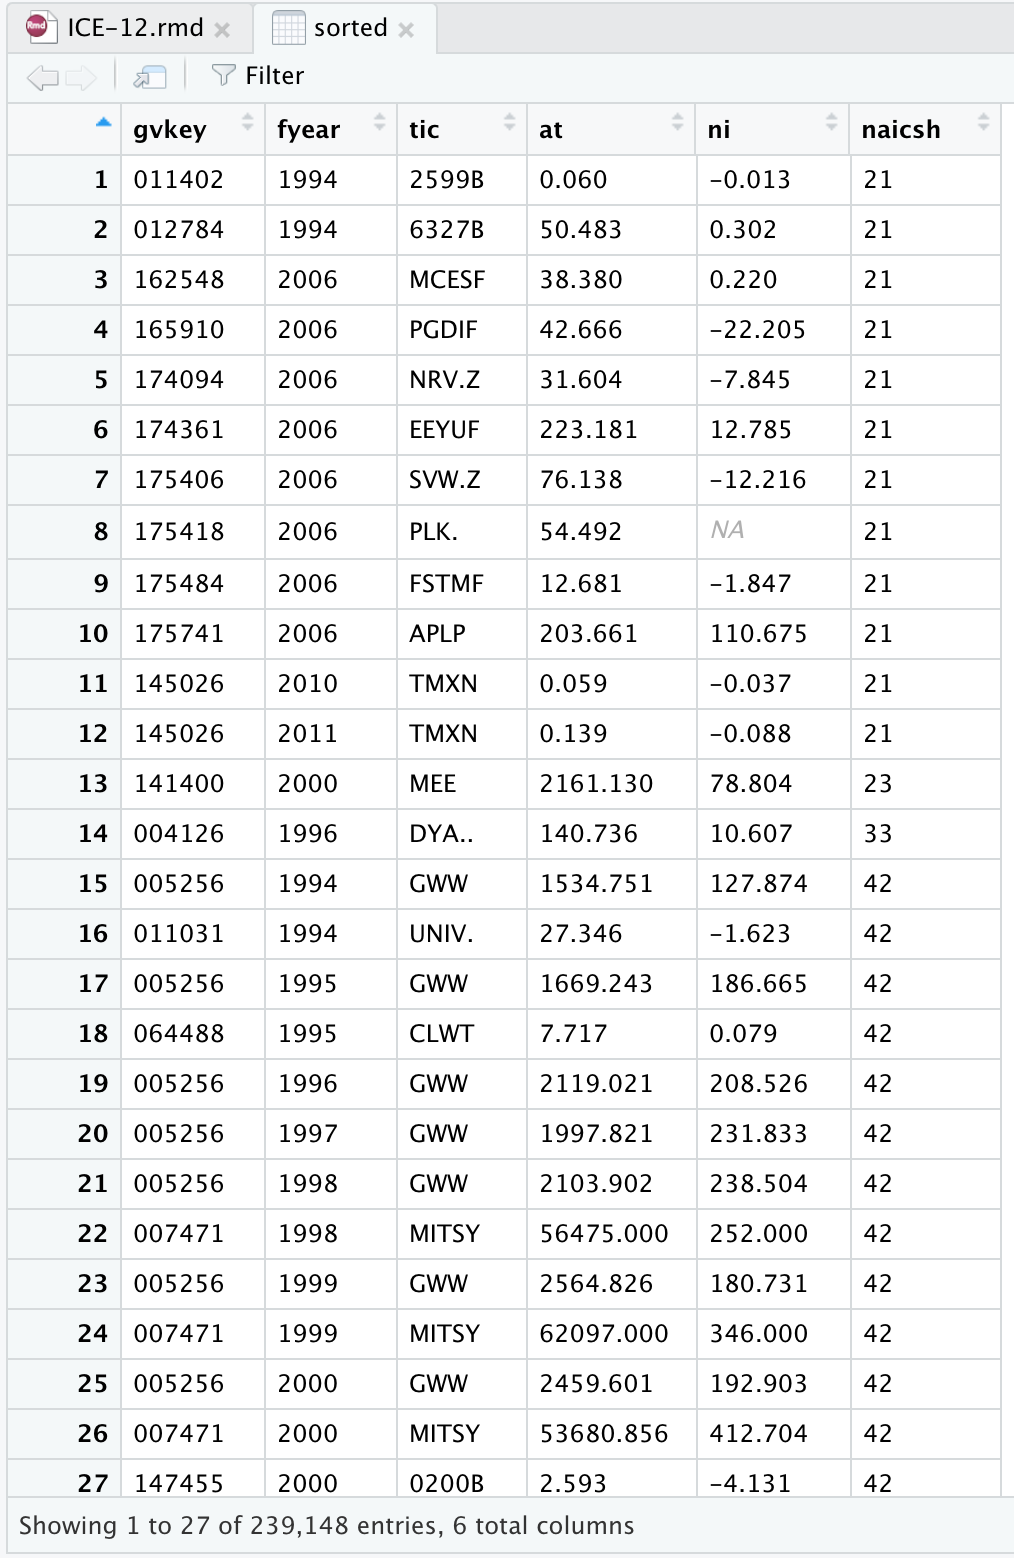
\includegraphics[width=0.8\textwidth]{./q5.png}
\end{center}


Looking at the image we can see it's pretty clearly sorted by \texttt{naicsh}, which is the North American Industry Classification System (NAICS) code identifier, in ascending order, but less obviously it also appears to be sorted by fiscal year in ascending order, within each NAICS code, and then on top of that it's sorted by \texttt{gvkey} within each fiscal year.  So we'd sort first by \texttt{naicsh}, then by \texttt{fyear}, and then by \texttt{gvkey} in that order.

You could just run each code snippet to see which one produces output like the image but you can just look and see that only answer B will actually do a sort, subsort, and sub-subsort in the correct order.  Answer A does the correct sorting but in the wrong order.  Answer F might come close but because you're piping each sort operation into the next what it does is just sort the dataframe three times without doing sub-sorts.   So, the answer is B.

\subsection*{Question 6, 1.25 pts}
\label{sec:org3b3dca6}
The default sort order is ascending, so what this code is doing is sorting by \texttt{a}, ascending, and then either sorting by \texttt{b} ascending or descending within each \texttt{a}.  This implies:

\begin{enumerate}
\item if \texttt{a} has no duplicates then we can only sort \texttt{b} one way, since there's only one \texttt{b} for any given \texttt{a}, so we tick the box for answer A.
\item if \texttt{b} has all identical values, then since we're sorting \texttt{a} the same way each time, it there's only one way to sort \texttt{b} irrespective of how \texttt{a} is sorted, so we tick the box for answer D
\end{enumerate}


The other answers are insufficient (this question reminds me of the GMAT, haha)

\newpage
\subsection*{Question 7, 1.25 pts}
\label{sec:org7c68d0d}
Starting with \texttt{companies} we'll drop all rows that have \texttt{at < 100} or \texttt{sale < 100} and we'll drop any rows with missing employment, sales, or assets.  Then after that we'll \texttt{group\_by()} company (aka \texttt{gvkey}) and compute average employment per firm where \texttt{loc==USA} in fiscal years 2016, 2017, and 2018.  The question asks how many firms would be included in this calculation.  Let's find out.  Reminder that filtering returns rows where the condition is true, so we need to invert some of these inequalities.

\begin{minted}[,frame=single]{r}
  q7 = companies %>%
    filter(!is.na(emp), !is.na(sale), !is.na(at)) %>%
    filter(at >= 100 | sale >= 100) %>%
    filter( (fyear <= 2018) & (fyear >= 2016) ) %>%
    filter(loc == "USA") %>%
    group_by(gvkey)

n_distinct(q7$gvkey)
\end{minted}

The question asks how many companies there are, but because we're filtering by multiple fiscal years we'll end up with an inflated count if we just use \texttt{nrow()} so instead we'll count the number of unique \texttt{gvkey} values using \texttt{n\_distinct()} which gives:

\begin{verbatim}
4181
\end{verbatim}

\subsection*{Question 8, 1.25 pts}
\label{sec:orgb0903fd}
This question is worded very confusingly.  I had no idea what it was even asking for, so thank you to my awesome classmates for interpreting.  Apparently "average per firm" means "take an average of each firms' employment figures in the 3 year period, then average those all together".  So, here that is:

\begin{minted}[,frame=single]{r}
q8 = q7 %>%
  mutate(avgemp = mean(emp)) %>%
  summarize(avgavg = mean(avgemp)) %>%
  summarize(avgavgavg = mean(avgavg))
\end{minted}

So assuming that's what the question meant it's 10.4 thousand.

\begin{verbatim}
10.4146899465838
\end{verbatim}
\end{document}